\documentclass[12pt]{article}
\usepackage[hmargin=2.0cm,vmargin=1cm]{geometry}
\usepackage[utf8]{inputenc}
\usepackage{graphicx}
\usepackage{float}
\usepackage{cite}
\usepackage{natbib}
\usepackage{amsmath}

\title{\begin{LARGE}
{Modelling the Milky Way dark matter halo}
\end{LARGE}}
\begin{document}
\maketitle

\section{Introduction}

In the current cosmological standard paradigm about 23\% of the energy and matter
content of the Universe is dark matter and $\sim 1\%$ is barionic matter. In the
context of galaxy formation where structure grows hierarquicaly, barionic matter
start to cluster inside dark matter halos where galaxies start to form. Therefore
studing the properties of these dark matter halos lead to a better understanding
of the galaxy formation processes. In particular the morphology, kinematics, dynamics
and formation history of galaxies are strongly related with the host dark matter halo. 

     
Crucial theoretical efforts have been made in order to model these dark matter halos 
properties. Hernquist, Plummer, Dehnen, derived analytical expresions for the density 
profiles of spherical dark matter halos. Using cosmological simulations Navarro et al 
found an analytical expression for DM profiles in a cold dark matter universe, they also 
study spherical cuspy halos. More recent studies have suggested that halos in a 
$\Lambda CDM$ Universe are triaxial Jung\& Suto 01.   

Satellite galaxies and globular clusters that orbit around the host halos would give 
a hint about the mass of the halo if the the position, line of sight velocities and tangential velocities
were known. such observations have been made for several objects around the milky way and 
different groups have constrain the mass of the milky way but there is not a consistent 
agreement.  

Due to the dynamical friction satellite galaxies and orvits would decay into the halo of the MW. During this 
process the satellite galaxy would be disteroyed leaving tidal streams \citep{toomretoomre72}
this streams where expected to be observed in the Milky Way \citep{lblb95, jhonston96}. 
The first satellite galaxy observed inside the Milky Way halo was the Sagittarius dSPh \citep{ibata94} 
and the streams were observed \citep{ivezic00, yanny00, ibata01b}. A full observation 
of the stream was made by \citep{majewsky03}, the stream  have a width ($>20°$) \citep{belokurov06} and it warps
for more than $360°$\citep{majewsky03, piladiaz13, belokurov14} around the milky way, 
the velocity space is ($>20km/s$) \citep{koposov13} this charactersitics suggest that
the Sgr stream is hot. 

The amount and precise observation of the Sgr stream have lead to test dark matter models of
the Milky Way due to the distances, radial velocities and the positions of
the stars. Several groups have attempt to reproduce the stream, (Ibata et al 01 (Spherical)
,Helmi 04 (Prolate), Johnston et al 05 (Oblate halo), Law et al 05,Fellhauer et al 06 (Spherical)
, Martinez Delgado et al 07 (Oblate), Law, Majewski, Johnston 09, Law \& Majewski (Triaxial),
Vera-Ciro 2013, These models are explained in detail in \S \ref{mw}. Despite these efforts
there is not a concistent model that fully reproduce the Sagitarius stream.

More recently Pearson14 used the Palomar 5 stream which is closer in order to test
the previous models at a different radius. They found that none of the previous
triaxial models can reproduce the Palomar 5 stream. Also the point that stream-fanning 

In all of the above efforts the halo is model as a static halo...


The LMC ...



\begin{itemize}
\item First observed by Ibata 94
\item Large population of young relatively metal rich Sgr M-giant wrapping 360
across the sky  (Majewski 03)
\item debris streamer continues through the North Galactic Pole passes over the 
solar neighborhood toward the galactic anitcenter. (Belokurov 06)
\item Evolution in metallicity distribution function.
\end{itemize}

Efforts trying to modelled the stream.

\begin{itemize}
\item Johnston 95, 99
\item Velazquez \& White 95
\item Edlesohn \& Elmegreen 97
\item Ibata et al 07
\item Gomez-Flechoso et al 99
\item Helmi \& White 2001
\item Martinez-Delgado et al 2004
\end{itemize}

MW DM halo:

\begin{itemize}
\item Ibata et al 01 (Spherical)
\item Helmi 04 (Prolate)
\item Johnston et al 05 (Oblate halo)
\item Law et al 05
\item Fellhauer et al 06 (Spherical)
\item Martinez Delgado et al 07 (Oblate)
\item Law, Majewski, Johnston 09 ()
\item Law \& Majewski (Triaxial)

\end{itemize}

\section{The Milky Way Dark Matter halo}\label{mw}
\subsection{Vera Ciro13}

\citep{Vera13} study a dark matter halo that is oblate in the center
 and triaxial in the outskirts. 

This study is motivated by expectations that the disk would modify the 

The motivations are that the disk is expected
 to modify the

 inner halo shape towards one that is oblate, in which case disk stability 
is ensured.  

also if the
halo is oblate at the inner the disk stability is ensured. 

They
argue that the triaxial halo configuration of \citep{Law10} it's
not common in the LCDM model due to the small c/a ratio compared to
LCDM predictions.

*** Is this actually an issue - can’t the MW be an outlier?   
***  How much of an outlier is the Law model vs average properties


They integrate orbits of test particles in the potential Eq.\ref{eq:vera} for a period
of 2gyr backwards and forwards. 

For every test particle they select 10 random locations 
in its orbit and store the position and velocity. 
orbit of this test particle from which they have positions and velocities.

 With this methodology they reproduce observables that might be compared with 
the Sgr stream.

The results from this numerical experiment is that 

They find  a good fit in some
parts of the orbits (see Fig.2 of that paper) and that the fit does not depend
strongly on the parameter $r_a$ of the halo potential.

In the second part of this paper they study the effect of torques in the Sgr
stream. The authors argue that there are two torques, one from the triaxiality
of the halo itself and the other due to the LMC. Interestingly, the major
axis of the triaxial potential in \citep{Law10} is in the direction towards
 the LMC. They studied the magnitude of both torques and found that both
have an equal effect on the Sgr stream.

As a result, they modify the parameters of the halo model in order to account
for the additional torque of the LMC, these new parameters are now more consistent
 with those expected from the LCDM model. For the orbit integration they also take
into account the potential of the LMC. With these considerations, they find a better fit for  the Sgr
stream (see Fig.5 of that paper).

\section{How common is the Milky Way}

\subsection{There’s no place like home? Statistics of Milky Way-mass dark matter
haloes (MBK10)}

The MW dark matter halo range between [$1\times 10^{12} - 3\times 10^{12}$]
typical $Rvir = 200 h^{-1}$. It is not common to have large satellites as
the MW. 

\subsection{The shape of the gravitational potential in cold dark matter haloes (Hayashi07)}

Goal: Study the shape of the gravitational potential of CDM halos. Radial dependence of triaxilaity in the potential of CDM halos.
 
Main Results: Near the center the halo is prolate $c/a = 0.72 \pm 0.04$
and $b/a = 0.78 \pm 0.08$. in the outer regions the halo is more sphereical.

Method: Simulate 7 MW sized halos and 4 dwarf galaxies and meauser the b/a, c/a ratios at $z=0$
\subsection{Meausuring a, b, c.}

Rememer $c<b<a$

\subsection{Halo shapes}

The monopole dominates in the outer regions of a centrally conentrated mass distribution, the n in the outer
regions the potential is more spherical. 

\begin{equation}
T = (a^2 - b^2)/(a^2-c^2)
\end{equation}

\begin{itemize}
\item $T=0$ -> Oblate
\item $T=1$ -> Prolate 
\end{itemize}


\begin{figure}[H]
\centering
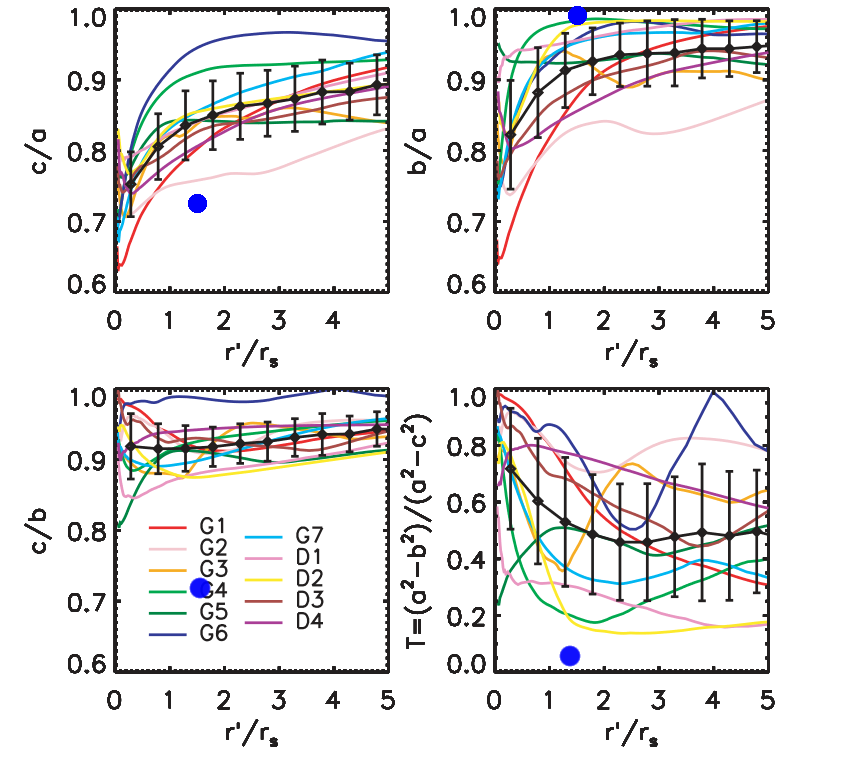
\includegraphics[scale=0.5]{hayashimod.png}
\end{figure}

\begin{figure}[H]
\centering
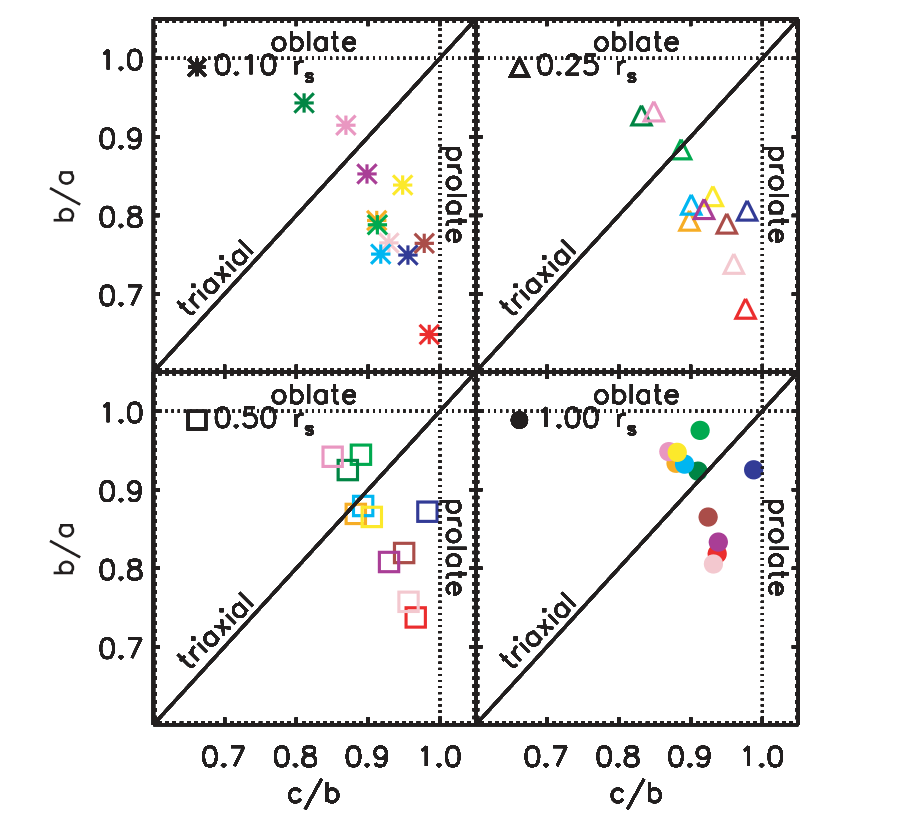
\includegraphics[scale=0.5]{prolateoblatehayashi.png}
\end{figure}


From the figure:

\begin{itemize}
\item c/b is almost constant. 
\end{itemize}

\textbf{They study 7 galaxies how is this statistically significant?, always 3 galaxies are outside the error bars }

The MW values according to \citep{Law10} are: $c/a = 0.72$ $b/a = 0.99$, $c/b = 0.72$, $T=0.042$

\subsection{The shapes and alignments of dark matter halos Schneider, D(2012)}

They study halos from $z=0-1$

Halos: they can resolve down to the $10\%$ of the virial radius. They use MilleniumI \& II.

$a<b<c$

$s=a/c$, $q=b/c$
  
For the MW this is: $s = 0.72 $, $q = 0.99 $


\begin{figure}[H]
\centering
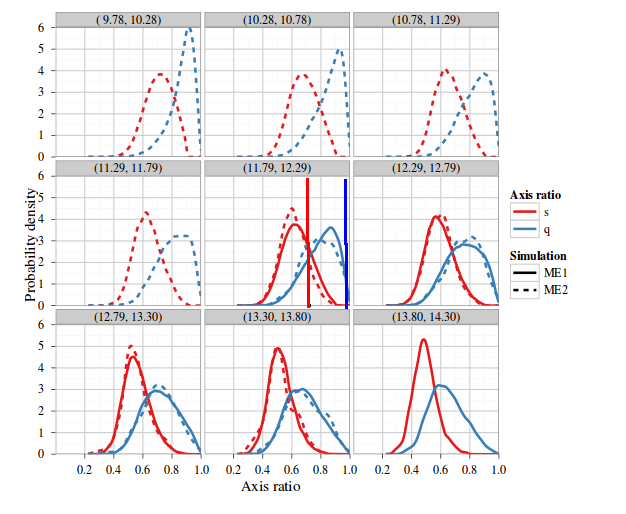
\includegraphics[scale=0.5]{distribution.png}
\end{figure}

\begin{figure}[H]
\centering
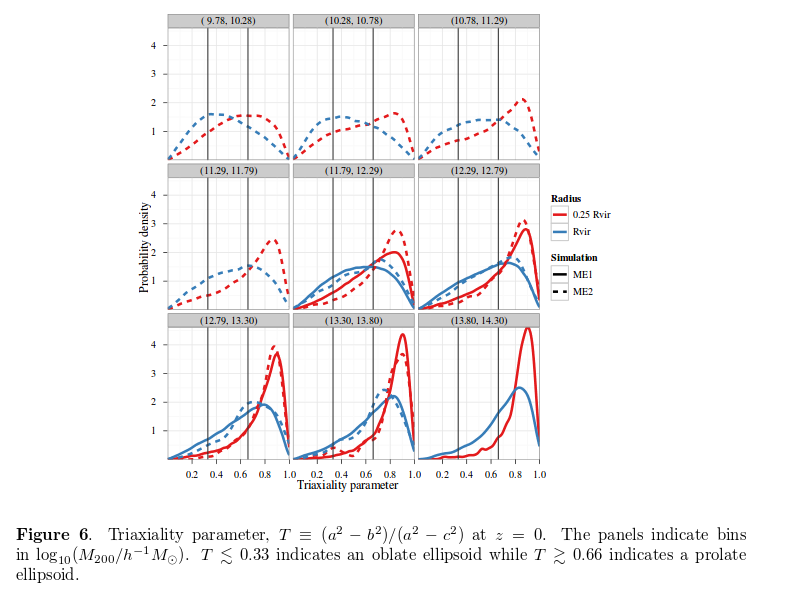
\includegraphics[scale=0.5]{triaxial.png}
\end{figure}


\subsection{Illustris halos}

\begin{figure}[H]
\includegraphics[scale=0.5]{illustris.pdf}
\end{figure}

\textbf{conclusion: Halos are more oblate in the center and at the outskirts are more triaxials}


\subsection{How the shape changes in time: (Vera-Ciro2011)}

Goal:  Determine the shape of the MW Dark Matter halo.

Main Results: individual halos changes with time, from prolate at earlier times 
to triaxial/oblate at present time measured in the virial radius. The halo 
shope is affected by accretion processes, if accretion is due to filaments
the halo tends to be more prolate. When the accertio is more isotropic the halo
is triaxial/oblate. The shape of the Dark Matter halo at diffeent radii shows 
the accertion history of the halo.    






\section{Alignments}

\subsection{Hayashi}

Angle between the principal axes of the isopotential and the corresponding
axis at larger radii. Solid lines show the results when the length of the 
axis differ from more than 5 percent, while dashed lines for axes with 
less tan 5 percent of length difference.

The main results are that in almost all the cases the 7/11 the axes are 
well aligned as a function of radii. (Why this happens?)

Minor axis in 6/11 tend to be alligned wih the total angular momentum vector 
(better that 25° at $r=5r_s$), disks would tend to form on the plane of 
the major and intermediate aes of the halo. In prolate halos this plane
doesn't have circular symmetry.


\begin{figure}
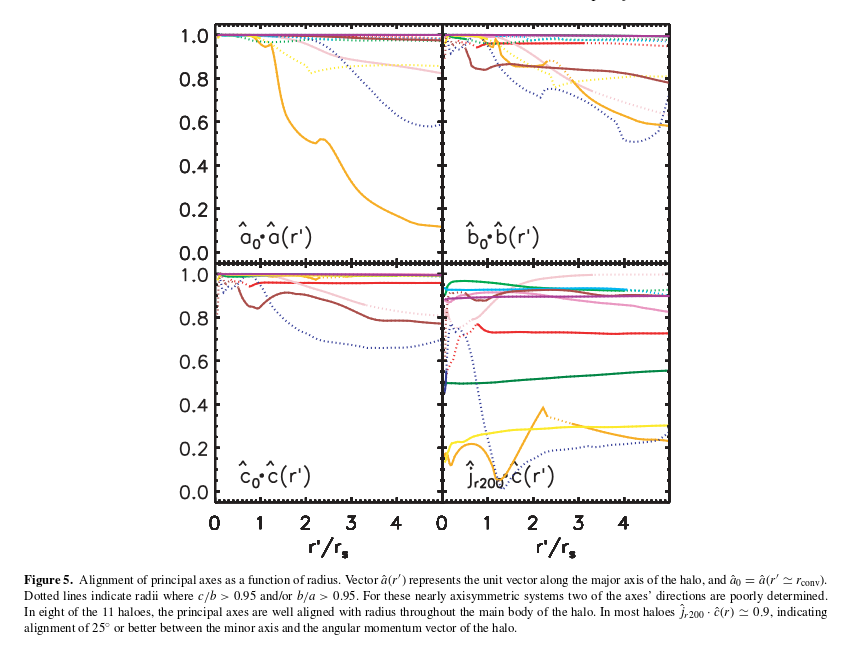
\includegraphics[scale=0.5]{alignmentH.png}
\end{figure}		

Most of the halos show a well alignment as a function of radius. 
Regarding the alignemnt of the potential with the angular momentum, they 
found that the minor axis tends to be alignment with the angular 
momentum vector 6 of 11 by $<25$. This is important because discs tend 
to be align with the halo's angular momentum. 

\subsection{Schneider et al, 2012}

Using the reduced inertia tensor (which reduces the effect to the alignment
in comparison with the non-reduces intertia tensor) to measure halo 
shapes for halos
at $z=0.5$ in the Millenium I and II simulations. \citep{scheider12}
found that halos major axis alignment tend to be perpendicular to the outskirds
of the halos.  

\begin{figure}[H]
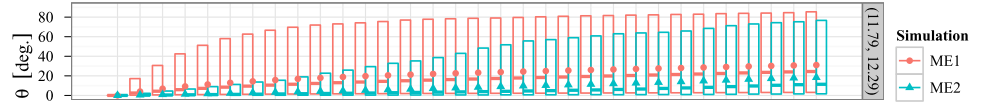
\includegraphics[scale=0.5]{schneideralignments.png}
\end{figure}

\citep{schneider12} also argue that the main difference between the 
Millenium I and II simulatios are due to the difference in resolution 
between the simulations. In Millenium I subhalos in the inner part 
of the halos are not resolved which makes that the angle between 
tha mayor axis increase. 

\section{Questions}

1. Is the MW common in LCDM
2. What is the $\hat{L}$ of the MW, is it common in LCDM?
3. Is the triaxial shape of the DM halo related with the large
scale structure in which the MW is embeded.


\section{Numerical Simulations}

\bibliographystyle{unsrtnat}
\bibliography{referencesDMMW}


\end{document}

